\hypertarget{_circle_8cpp}{
\section{src/util/Circle.cpp File Reference}
\label{_circle_8cpp}\index{src/util/Circle.cpp@{src/util/Circle.cpp}}
}


\hyperlink{class_circle}{Circle} Class.  


{\ttfamily \#include \char`\"{}../../include/tester/util/Circle.h\char`\"{}}\par
{\ttfamily \#include $<$GL/glut.h$>$}\par
Include dependency graph for Circle.cpp:\nopagebreak
\begin{figure}[H]
\begin{center}
\leavevmode
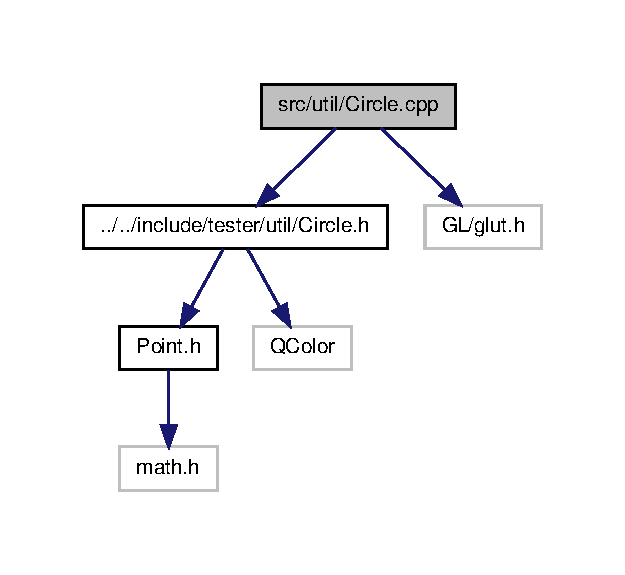
\includegraphics[width=300pt]{_circle_8cpp__incl}
\end{center}
\end{figure}


\subsection{Detailed Description}
\hyperlink{class_circle}{Circle} Class. \begin{DoxyAuthor}{Author}
Miguel Alejandro Parra Romero (\href{mailto:maparrar@unal.edu.co}{\tt maparrar@unal.edu.co}) 

Jean Pierre Charalambos 

Universidad Nacional de Colombia -\/ 2011
\end{DoxyAuthor}
BSD License

Project info \href{http://code.google.com/p/tester-device/}{\tt http://code.google.com/p/tester-\/device/} 

Definition in file \hyperlink{_circle_8cpp_source}{Circle.cpp}.

